
\section{Limits and Continuity}

\subsection{Introduction to the concept of limit}
\begin{minipage}{0.65\textwidth}
    We can conceptualize that the limit of a function $f(x)$ is $L$ as $x$ approaches $c$, given that we can make $f(x)$ \emph{as close to $L$ as we want} for all $x$ sufficiently close to $a$, from both sides, \emph{without actually letting $x$ be $a$}. We can write this as:
    \[\lim_{x\to a}f(x)=L\]
\end{minipage}
\hfill
\begin{minipage}{0.3\textwidth}
    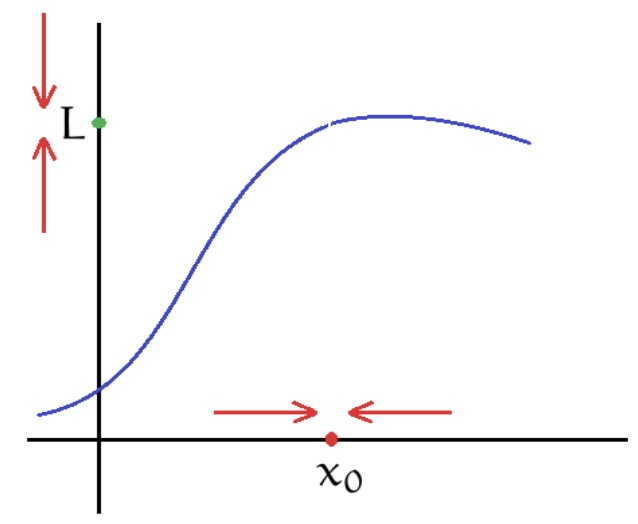
\includegraphics[width=\textwidth]{img/Lim.jpg}
\end{minipage}

\subsection{One-sided limits}
There are two sides that $x$ can tend to a number. We can write it as $x\to n^-$ and $x\to n^+$, which represents from the negative (left) / positive (right) side.

\subsection{Existence of limits}
\begin{theorem}
    {Condition for limit to exist}
    The limit for a function $f(x)$ only exists if and only if:
    \[\lim_{x\to a^+}f(x)=\lim_{x\to a^-}f(x)\]
    WARNING: If the \textbf{limit is} $\mathbf{\infty}$ it \textbf{doesn't exist}.

\end{theorem}

\begin{minipage}{0.65\textwidth}
    For this example, when $x\to 0^-, y\to -\infty$.

    Similarly, as $x\to 0^+, y\to +\infty$.

    Hence, we can conclude that the limit for this function as $x\to 0$ doesn't exist.
\end{minipage}
\hfill
\begin{minipage}{0.25\textwidth}
    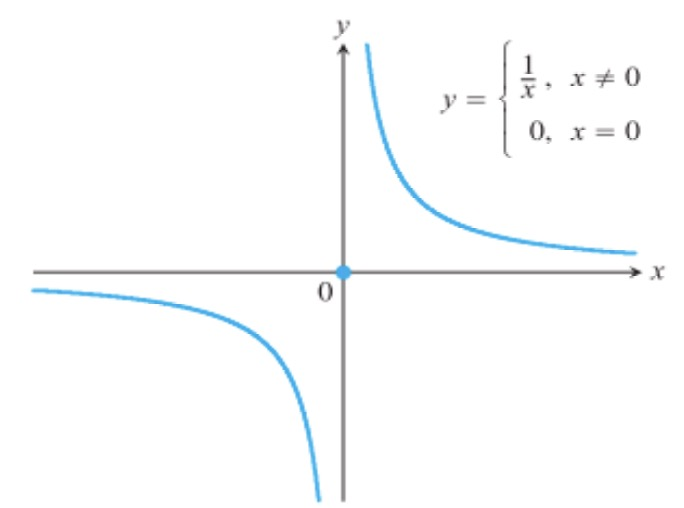
\includegraphics[width=\textwidth]{img/lim3.jpg}
\end{minipage}

\subsection{Continuity}
\begin{definition}
    {Continuity}
    A function $f(x)$ is \emph{continuous} at $x=a$ if:
    \[\mathop {\lim }\limits_{x \to a} f\left( x \right) = f\left( a \right)\]
\end{definition}
\begin{knBox}
    {Continuity properties}
    For $f,g$ continuous at $c$, the following are also continuous at $c$:
    \begin{enumerate}
        \item $f \pm g$
        \item $kf$
        \item $fg$
        \item $\frac{f}{g}$, given that $g(c)\ne 0$
    \end{enumerate}
\end{knBox}
\begin{theorem}
    {Intermediate value theorem (IVT)}
    If a function $f$ is continuous on $[a, b]$, there is a number $c$ in $[a, b]$ where $f(c)$ in $[f(a), f(b)]$.

    We use the IVT by first finding $f(a)$ and $f(b)$, then apply the rule.
    \tcblower
    To prove that there is a root, we can use the IVT by showing there is a \textbf{change of sign} between the interval given.
\end{theorem}

\subsection{Computing limits}
\label{sec:indeterminate}
\begin{definition}
    {Indeterminate forms}
    Indeterminate forms are forms that cannot be solved by simply substituting the value of $x$ into the function. They are:
    \[\frac{0}{0},\quad\frac{\infty}{\infty},\quad0\cdot\infty,\quad\infty-\infty,\quad\infty^0,\quad1^\infty,\quad\infty^0\]
    Note that $\infty + \infty = \infty$. Related: \hyperref[sec:lhr]{L'Hopital's rule}
\end{definition}
\begin{theorem}
    {Using the limit laws}
    For functions $f,g$ and using $\mathop {\lim }\limits_{x \to a}=\bigcirc$ for simpler notation:
    \begin{enumerate}
        \item $lim_{x\to a}c=c$
        \item $\bigcirc(f\pm g)=\bigcirc f\pm \bigcirc g$
        \item $\bigcirc(k\cdot f)=\bigcirc k\cdot\bigcirc f$
        \item $\bigcirc(f^n)=(\bigcirc f)^n$
        \item $\bigcirc(fg)=\bigcirc f\bigcirc g$
        \item $\bigcirc(\frac{f}{g})=\frac{\bigcirc f}{\bigcirc g},\quad\text{given that }\bigcirc g\ne 0$. \emph{This strict condition prevents indeterminate forms.}
    \end{enumerate}
    We can use these laws to break a limit into separate limits, and compute that way. Also note that:
    \begin{enumerate}[start=7]
        \item $\bigcirc f(g)=f(\bigcirc g),\quad$given that $f$ is \textbf{continuous} at $\bigcirc g$
    \end{enumerate}
\end{theorem}
\begin{theorem}
    {Limit of a polynomial}
    For the limit of a polynomial $p(x)$:
    \[lim_{x\to a}p(x)=p(a)\]
    This can be proven easily with the limit laws above.
\end{theorem}
\begin{knBox}
    {Techniques to compute limits}
    To solve for limits, we have to get the expression to the right form - a polynomial, for us to substitute our limit value into the function.

    To do this, often we have to \textbf{factorize} or \textbf{rationalize}.
\end{knBox}
\begin{knBox}
    {Limits of composite functions}
    For the limit of a composite function $\lim_{x\to a}f(g(x))$, where $f$ is \textbf{not} continuous at $g(a)$, we find $b$ as $x\to a,g\to b$, and then find $\lim_{x\to b}f(x)$ at that value.

    The following explains some common cases:
    \begin{enumerate}
        \item $x\to a^-, g\to g(a)^-$
        \item $x\to a^-, -x\to -a^+$
    \end{enumerate}

    For $y=\lim_{x\to a}f(x)^{g(x)}$, we can the logarithm to simplify the function, and determine $\lim_{x\to a}\ln y$ and find $\lim_{x\to a}y=e^{\lim_{x\to a}\ln y}$.
\end{knBox}
\begin{knBox}
    {Limits of square roots}
    To solve for limits of square roots, we can multiply by the conjugate to rationalize the function.
    \[\lim_{x\to a}f(x)+\sqrt{g(x)}=\lim_{x\to a}\frac{f^2(x)-g(x)}{f(x)-\sqrt{g(x)}}\]
\end{knBox}

\begin{theorem}
    {The squeeze / sandwich theorem}
    Suppose $f(x)\le g(x) \le h(x)$ in the range $[a, b]$, for $c$ in $[a, b]$:
    \[\lim_{x\to c}f \le \lim_{x\to c}g \le \lim_{x\to c}h\]
    We will make use of the fact that the limits can be equal to solve for the limit of $g(x)$.
\end{theorem}

\begin{example}
    Squeezing a function

    When we can't seem to factorize a function, we can try squeezing it between two other functions.
    \[\lim_{x\to 0}x^2\cos\frac{1}{x}\]
    We know the limits of the function $\cos \frac{1}{x}$, so we can start from there.
    \[\text{Given that }x\ne 0, -1\le \cos \frac{1}{x} \le 1\]
    \[\text{Multiplying }x^2\text{ on both sides},-x^2\le \cos x^2\frac{1}{x} \le x^2\]
    \[\text{As }\lim_{x\to 0}\pm x^2=0,\quad\text{we can conclude that }\lim_{x\to 0}x^2\cos\frac{1}{x}=0\]
\end{example}

\subsection{Infinite limits}
\begin{knBox}
    {Determining infinite limits}
    If $f(x)$ gets (negatively) arbitrarily large when $x$ approaches $a$, we can say:
    \[\lim_{x\to a}f(x)=(-)\infty\]
    After we know that the limit \emph{may} be infinity, we then have to make sure that \emph{the limit is the same from both sides}, so that the limit is actually $\infty$. We can do so by plugging numbers which are approaching the limit from both sides.
\end{knBox}

\begin{minipage}{0.45\textwidth}
    \begin{example}
        Infinite limit exists
        \[\lim_{x\to 0}\frac{6}{x^2}\]
        \[\text{Consider both}\ \lim_{x\to 0^-}\frac{6}{x^2},\lim_{x\to 0^+}\frac{6}{x^2}:\]
        \[\lim_{x\to 0}\frac{6}{x^2}=\infty\]
    \end{example}
\end{minipage}
\hfill
\begin{minipage}{0.45\textwidth}
    \vspace{10pt}
    \begin{example}
        Infinite limit doesn't exist
        \[\lim_{x\to 4}\frac{3}{(4-x)^3}\]
        \begin{center}
            Checking both sides, we can conclude that the limit doesn't exist, as:
        \end{center}
        \[\lim_{x\to 4^+}\frac{3}{(4-x)^3}=-\infty,\quad\lim_{x\to 4^-}\frac{3}{(4-x)^3}=\infty\]
    \end{example}
\end{minipage}

\subsection{Limits at infinity}
\begin{theorem}
    {Infinity operations}
    Note the following operations:
    \begin{enumerate}
        \item $\infty + k=\infty$
        \item For $k<0,\ k\infty=-\infty$
        \item $-\infty\times\infty=-\infty$
    \end{enumerate}
\end{theorem}
\begin{knBox}
    {Determining limits of infinity}
    It is not hard to see that, for rational numbers $n$:
    \[\lim_{x\to\pm\infty}\frac{k}{x^n}=0\]
    The easiest way to determine the limit would be to \emph{factorize} the function so that we can use the fact above.
\end{knBox}
\begin{theorem}
    {Determining limits of infinity of polynomials}
    Using the above fact, we can see that for a polynomial $p(x)$ with degree $n$ and largest coefficient $a_n$:
    \[\lim_{x\to\pm\infty}p(x)=a_nx^n\]
    Which means we can \emph{only consider the largest term in a polynomial} for limits of infinity.
\end{theorem}
\begin{example}
    Indeterminate forms by substitution of infinity

    Substituting $\infty$ into the function gives $\infty-\infty-\infty$, which is indeterminate. Hence, we must factorize it.
    \begin{align*}
        \lim_{x\to\infty}2x^4-x^2-8x & =\lim_{x\to\infty}[x^4(2-\frac{1}{x^2}-\frac{8}{x^3})] \\
                                     & =\infty\times 2                                        \\
                                     & =\infty
    \end{align*}
    Or we can just simply use the theorem above and consider $\lim_{x\to\infty}2x^4$ only to give $\infty$.
\end{example}
\begin{example}
    Factor polynomials limit to infinity

    We can simply consider the largest terms on each side and give the final answer easily.
    \begin{align*}
        \lim_{x \to -\infty } \frac{{\sqrt {3{x^2} + 6} }}{{5 - 2x}} & =\lim_{x \to -\infty }\frac{\sqrt{3x^2}}{-2x}                           \\
                                                                     & =\lim_{x \to -\infty }\frac{\sqrt{3}|x|}{-2x} \leftarrow \sqrt{x^2}=|x| \\
                                                                     & =\lim_{x \to -\infty }\frac{-\sqrt{3}}{-2} \leftarrow |c|,c<0=-c        \\
                                                                     & =\frac{\sqrt{3}}{2}
    \end{align*}
    Note that, as we are considering the negative limit of infinity, we need to add - to the abs sign on line 3.
\end{example}

\label{sec:asymptotes}
\subsection{Asymptotes}
\begin{definition}
    {Vertical asymptotes}
    $f$ will have v-asymptotes at $x=a$ if any $\pm$ is true:
    \[\lim_{x\to a^\pm}f(x)=\pm\infty\]
\end{definition}
\begin{definition}
    {Horizontal asymptotes}
    $f$ will have h-asymptotes at $y=L$ if any $\pm$ is true:
    \[\lim_{x\to\pm\infty}f(x)=L\]
\end{definition}
Related: \hyperref[sec:graph]{Graphing functions}